\documentclass[12pt]{article}

\usepackage{sbc-template}

\usepackage{graphicx,url}

\usepackage[brazil]{babel}   
%\usepackage[latin1]{inputenc}  
\usepackage[utf8]{inputenc}  
% UTF-8 encoding is recommended by ShareLaTex
\usepackage[none]{hyphenat}
\usepackage{url}

\sloppy

\title{Técnica anti-forense: esteganografia em imagens}

\author{Leonardo G. Carvalho\inst{1}, Matheus S. Redecker\inst{1}}


\address{Pontifícia Universidade Católica do Rio Grande do Sul - PUCRS \\
Porto Alegre, RS - Brasil
  \email{  \{leonardo.gubert\}\{matheus.redecker\}@acad.pucrs.br}
}
\begin{document} 

\maketitle

\begin{abstract}
The steganography in images is the art of hiding information inside images. The steganography in images can be used to exchange confidential messages, or hide information from others. This work shows a description of the techniques used in the creation and detection of steganography.
\end{abstract}

\begin{resumo} 
A esteganografia em imagens é a arte de ocultar informações dentro de imagens. A esteganografia em imagens pode ser usada para troca de mensagens sigilosas, ou ainda esconder informações de terceiros. Este trabalho mostra uma descrição das técnicas usadas na criação e na detecção da esteganografia. 
\end{resumo}

\section{Introdução}
No passado, as pessoas usavam tintas invisíveis ou tatuagens escondidas para trocar informações sigilosas. Hoje em dia com os computadores e a internet, existem maneiras melhores de conseguir isso. Uma dessas maneiras é a esteganografia \cite{hideAndSeek}. Esteganografia é uma palavra que vem do grego e significa “escrita oculta” e consiste na arte ou ciência de se escrever mensagens ocultas de tal forma que ninguém saiba que essa mensagem exista. É diferente da criptografia em que a mensagem tem sua existência conhecida, mas não se sabe como decifrá-la \cite{newton}. A esteganografia vem se destacando muito no decorrer dos tempos e está ganhando popularidade com a Internet, para comunicação em segredo e para atender a atual demanda da indústria por marca d’água digital e impressão digital para áudio e vídeo \cite{tcc}. Arquivos como os de imagem e som possuem áreas de dados que não são usadas ou são pouco significativas. A esteganografia tira proveito disso, trocando essas áreas por outra informação \cite{ufrgs}. 

A esteganografia em imagens é obtida sabendo explorar as limitações do sistema visual humano (SVH). Ela evoluiu muito com o desenvolvimento de computadores gráficos rápidos e poderosos, além de que os softwares esteganográficos estão disponíveis para usuários diários da Internet \cite{tcc}. Uma imagem colorida é normalmente formada por um conjunto de pixels, nos quais suas cores são armazenadas em 3 ou 4 canais, sendo eles RGB (vermelho, verde e azul) ou RGBA (vermelho, verde, azul e alpha) respectivamente, cada canal contendo 8 bits (1 byte). Alterando-se o bit menos significativo de qualquer um dos canais não ocasiona-se mudanças perceptíveis na imagem. Desta forma, podemos trocar estes bits por uma outra sequencia (arquivo ou texto) usando apenas o bit menos significativo de um ou todos canais de cada pixel \cite{ufrgs, tcc}.

\section{Técnicas}

As técnicas mais comuns para fazer estas alterações envolvem o uso de \textit{least-significant bit} (LSB), \textit{filtering}, \textit{masking} e \textit{transformations}. Estas técnicas podem ser usadas com variados graus de sucesso em diferentes tipos de arquivos de imagem \cite{methods}. A distribuição das técnicas na imagem pode ser feita de forma sequencial, ou seja, do inicio da imagem para o final, linha por linha, de trás para frente, coluna por coluna.  

\subsection{Least Significant Bits}

As fotografias possuem uma quantidade significativa de ruído e esconder a informação que se deseja transmitir nesse ruído é, provavelmente, a técnica esteganográfica mais utilizada. Uma imagem pode utilizar diversas formas de armazenar a informação de cada pixel dependendo do formato com que foram exportadas. Uma imagem BMP por exemplo pode utilizar o formato RGB24 (24 bits/pixel, 8 bits para cada canal) ou até mesmo RGBA32 (32 bits/pixel, 8 bits para cada canal). Além do RGB, também existem imagens que trabalham com apenas 1 canal (\textit{grayscale}) ou com o formato CMYK (ciano, magenta, amarelo e preto, cada canal com 8 bits), normalmente utilizado para imagens que serão impressas.
A técnica dos \textit{Least Significant Bits} pode ser considerada a técnica mais simples, pois apenas utiliza o bit menos significativo de cada pixel da imagem, podendo usar o ultimo bit de cada canal para esconder as informações \cite{methods}. 

As mudanças que ocorrem na imagem com essa técnica são quase imperceptíveis pelo fato de que a alteração da tonalidade da cor é pequena demais para que o olho humano detecte a diferença. Além disso, em média apenas metade dos bits são alterados, o que deixa algumas cores totalmente inalteradas \cite{methods}.

Para uma melhor eficacia é recomendado usar essa técnica em imagens com formatos em que não sejam comprimidas, pois os algoritmos de comprimir imagens como o JPEG se aproveitam dos ruídos para eliminar algumas informações \cite{methods, tecnica}.

A figura \ref{comp} mostra duas imagens, a original a esquerda e a com esteganografia a direita, e nela pode ser visto que não há uma difereça perceptível. 

\begin{figure}[ht]
	\centering
	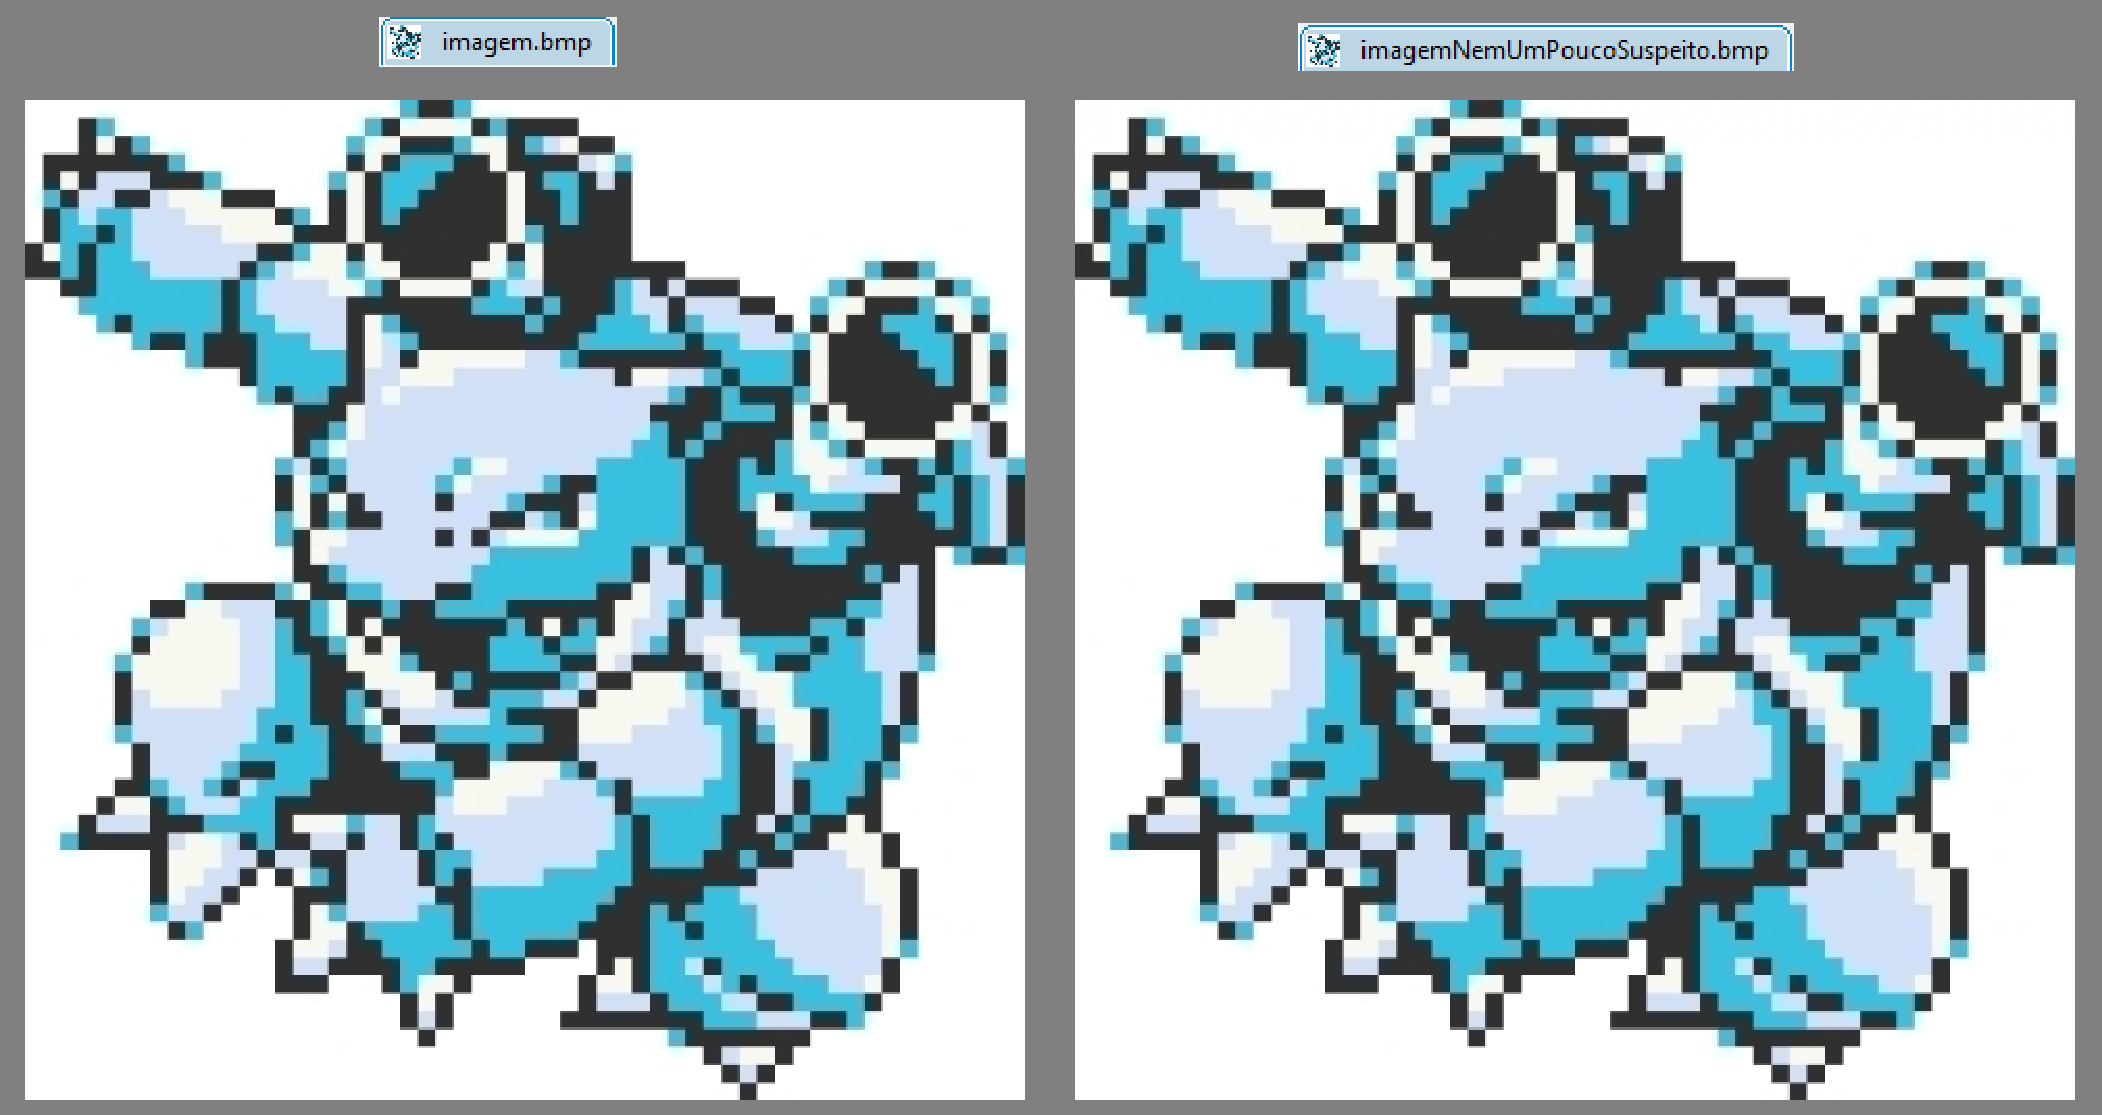
\includegraphics[width=0.6\textwidth]{imagens.pdf}
	\caption{Informação escondida com esteganografia dentro da imagem}
	\label{comp}
\end{figure} 

\subsection{Masking and filtering}

As técnicas de \textit{masking} e \textit{filtering} geralmente são utilizadas em imagens em tons de cinza (\textit{grayscale}). Estes métodos são semelhantes a marcas d\'agua, pois criam marcações na imagem alterando a luminância de algumas partes. As alterações são feitas sem que o olho humano consiga notar a diferença. \textit{Masking} utiliza aspectos visíveis da imagem, por esse motivo ela é mais robusta que a LSB e como a parte modificada não está nos ruídos, este tipo de técnica pode ser melhor empregado nas imagens de formato comprimidos, como JPEG \cite{methods}. A Imagem \ref{gray}\cite{wu2003} mostra um exemplo dessa conversão.

\begin{figure}[ht]
	\centering
	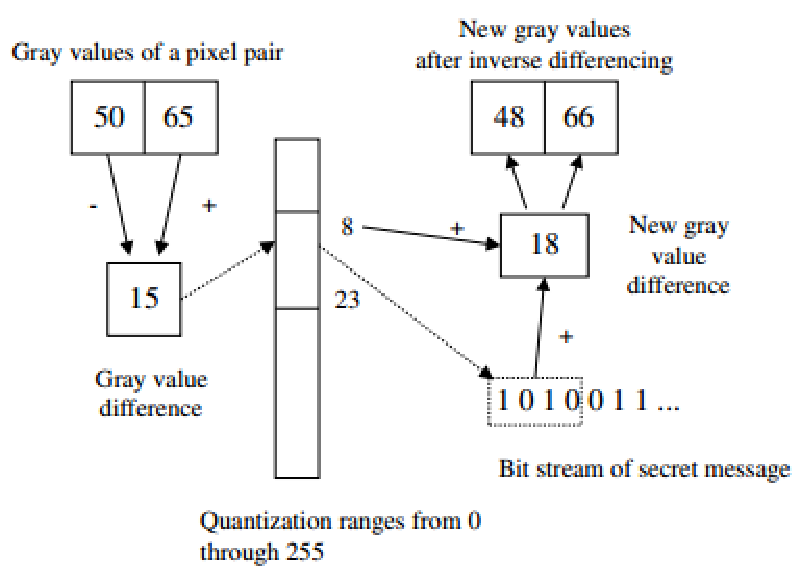
\includegraphics[width=0.6\textwidth]{mask.pdf}
	\caption{Masking and filtering}
	\label{gray}
\end{figure} 

\subsection{Transformations}

Uma forma mais complexa de esconder informação dentro das imagens vem de transformações discretas de cosseno. \textit{Discrete cosine transformations} (DCT) é usada para transformar blocos de 8x8 de uma imagem em 64 coeficientes de DCT. Cada coeficiente DCT F(u,v) de um bloco 8x8 de uma imagem com pixels f(x,y) é dado por \cite{methods}:

\begin{figure}[ht]
	\centering
	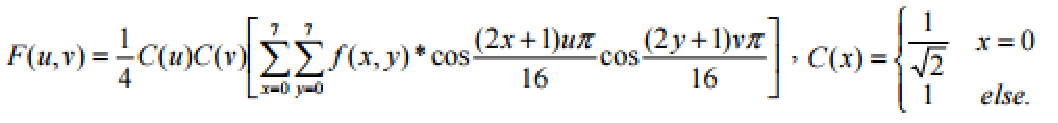
\includegraphics[width=0.8\textwidth]{formula.pdf}
\end{figure} 

\section{Esteganálise}

As técnicas de esteganografia não são totalmente perfeitas. Nenhuma delas garante que as informações escondidas não serão detectadas ou interceptadas por terceiros. A esteganálise busca utilizar métodos para detectar a esteganografia. A esteganálise pode buscar apenas verificar a existência de informações escondidas, sem estar preocupada em saber o conteúdo da mensagem, ou ainda recuperar os dados escondidos. Recuperar os dados adiciona um nível maior de complexidade ao processo de esteganálise, pois é necessário conhecer previamente o algoritmo de esteganografia utilizado. Além disso, a mensagem pode estar criptografada. As técnicas de esteganálise possuem algumas limitações. Muitas delas, por exemplo, foram feitas especialmente para determinados algoritmos e softwares de esteganografia que já são previamente conhecidos, e com isso se o algoritmo ou o software for diferente essa analise tem grande probabilidade de falhar \cite{tecnica}.

Após a descoberta de que há informação na imagem, pode-se ter diferentes objetivos em relação aos arquivos que ela contém. Os principais objetivos são:

\begin{itemize}
    \item Destruir a informação - Com o intuito de destruir a informação que está contida na imagem, pode-se destruir a imagem, ou para não danificar a imagem, pode-se adicionar novas informações com a ambição de colocar dados em cima dos dados anteriores, ou ainda, alterar o formato da imagem ou comprimi-la pode também destruir os dados que estão presentes.
    \item Obter a informação - Com o intuito de obter a informação que está contida na imagem, pode-se tentar utilizar algoritmos conhecidos para remontar a imagem. O problema vem do fato de que se a informação está criptografada, mesmo após descobrir o arquivo, tem o esforço para abrir-lo se for possível.
\end{itemize}

\section{Conclusão}

A partir da pesquisa desse trabalho podemos concluir que a esteganografia sempre altera a imagem original, e com isso é possível detectar a presença de esteganografia nas imagens. A diferença da imagem esteganografada para a original é tão pequena que não é perceptível ao olho humano. 

A esteganografia se torna uma aplicação interessante para troca de mensagens de forma sigilosa, pois quem abre a imagem de imediato não detecta nada de diferente. Para descobrir a informação escondida não é uma tarefa trivial, pelo fato das diversas técnicas existentes, e para extrair as informações é preciso saber qual a técnica foi usada para esconder a informação. Se além da esteganografia, a informação escondida estiver criptografada, é praticamente impossível descobrir a informação, o máximo que um interceptador consegue fazer é destruir a informação. 

Essa técnica é de fácil acesso e uma pesquisa rápida na internet já é possível conseguir um software pronto para usar. Um exemplo de software é o \textit{Hide \& Reveal}\footnote{http://hidereveal.ncottin.net/} e o software desenvolvido por nós para a demonstração do trabalho OEscondedor\footnote{https://github.com/Redecker/OEscondedor}.



\bibliographystyle{sbc}
\bibliography{sbc-template}

\end{document}
